\documentclass[journal,10pt,twocolumn]{article}
\usepackage{graphicx}
\usepackage[margin=0.5in]{geometry}
\usepackage[cmex10]{amsmath}
\usepackage{array}
\usepackage{booktabs}
\usepackage{mathtools}
\title{\textbf{Optimization Assignment - 2}}
\author{Lakshmi Kamakshi}
\date{September 2022}


\providecommand{\norm}[1]{\left\lVert#1\right\rVert}
\providecommand{\abs}[1]{\left\vert#1\right\vert}
\let\vec\mathbf
\newcommand{\myvec}[1]{\ensuremath{\begin{pmatrix}#1\end{pmatrix}}}
\newcommand{\mydet}[1]{\ensuremath{\begin{vmatrix}#1\end{vmatrix}}}
\providecommand{\brak}[1]{\ensuremath{\left(#1\right)}}
\providecommand{\lbrak}[1]{\ensuremath{\left(#1\right.}}
\providecommand{\rbrak}[1]{\ensuremath{\left.#1\right)}}
\providecommand{\sbrak}[1]{\ensuremath{{}\left[#1\right]}}

\begin{document}

\maketitle
\paragraph{\textit{Problem Statement} - Find the maximum area of an isosceles triangle inscribed in the ellipse \begin{align} \frac{x^2}{a^2}+ \frac{y^2}{b^2} = 1 \end{align}  with its vertex at one end of the major axis.} 

\section*{\large Solution}
\subsection*{\normalsize Gradient descent}
Let the lengths of major and minor axis of the ellipse be 4,3.
\begin{align}
	a = 4
	\\b=3
\end{align}
\\The equation of the ellipse and the major axis 
\begin{align}
	\vec{x}^T\vec{V}\vec{x} + f = 0 
	\label{eq:ellipse}	
\end{align}
where,
\begin{align}
	\vec{V} = \myvec{b^2&0\\0&a^2}
	\\f = -a^2b^2
\end{align}
major axis is
	\begin{align}
		\myvec{0&1}\vec{x} = \vec{0}
	\end{align}
\\Given one of the vertex is at one end of the major axis. The vertex will be $(a,0)$
\\let us assume 2 points on the ellipse , such that an isosceles triangle can be formed. The vertices of the triangle be,
\begin{align}
	\vec{x_1} = \myvec{a \\ 0} ;
	\vec{x_2} = \myvec{x_1 \\ x_2} ;
	\vec{x_3} = \myvec{y_1 \\ y_2} 
\end{align}
The height and side of the triangle  will be perpendicular to each other.The line vector of the height is the major axis of the ellipse
\begin{align}
           \myvec{0&1}\vec{x}=0
	 \\  \myvec{0&1}\myvec{x_1-y_1 \\ x_2-y_2} = 0
\end{align}
Upon simplification of the above dot product we arrive at,
\begin{align}
	x_1 = y_1
\end{align}
\\The given triangle is isosceles , thus 
\begin{align}
\vec{||x_1-x_2||} = \vec{||x_1-x_3||}
\end{align}
\begin{align}
\implies \vec{\sqrt{|x_1|^2+|x_2|^2-2x_1.x_2^T}} = \vec{\sqrt{|x_1|^2+|x_3|^2-2x_1.x_3^T}} 
\end{align}
\begin{align}
	\vec{\sqrt{|x_2|^2}} = \vec{\sqrt{|x_3|^2}}
	\\   \vec{x_2} = \pm \vec{x_3}
	\\ \myvec{ x_1 \\ x_2 } = \pm \myvec{ y_1 \\ y_2}
	\\  \myvec{x_1 \\ x_2} = \myvec{x_1 \\ \pm y_2}
	\\ y_2 = -x_2
\end{align}
if $+y_2$ is considered , the points will be same and cannot form a triangle.
\\The area of the triangle can be obtained from the cross product 
\begin{align}
	A = \frac{1}{2} \mydet{\vec{\brak{x_1-x_2}} \times \vec{\brak{x_1-x_3}}}
	\\ \implies \frac{1}{2} \mydet{a-x_1 & a-x_1 \\ x_2 & -x_2}
	\\ \implies \frac{1}{2} \brak{ \vec{2ax_2-2x_1x_2}}	
	\\ \vec{A} = \vec{ax_2-x_1x_2}
	\label{eq:Area}
\end{align}
The vertices of the triangle lies on the ellipse in \eqref{eq:ellipse}
\begin{align}
	\myvec{x &y} \myvec{b^2 & 0 \\ 0& a^2} \myvec{x \\y} = a^2b^2
	\\ y = \frac{b}{a}\sqrt{a^2-x^2}
	\label{eq:yval}
\end{align} 
\\Substitute \eqref{eq:yval} in \eqref{eq:Area} for the $x_2$ value. Thus , Area of the triangle  evaluates to  
\begin{align}
\implies A = b\sqrt{a^2-x^2} + \frac{b}{a}x\sqrt{a^2-x^2}
	\label{eq:f(x)}
\end{align}
The polynomial in \eqref{eq:f(x)} is the area of the isosceles triangle in one varible.The maximum area of the triangle will be found by finding the local maxima of the function.
Using gradient ascent method we can find its maxima ,
    \begin{align}
        x_{n+1} &= x_n + \alpha \nabla A \\
	    \implies x_{n+1} &= x_n + \alpha \brak{\frac{ba^2-2bx^2-abx}{a\sqrt{a^2-x^2}}}
    \end{align}
Taking $x_0=1,\alpha=0.001$ and precision = 0.0000001, values obtained using python are:
    
    \begin{align}
        \boxed{\text{Maxima} = 15.5885}\\
        \boxed{\text{Maxima Point} = 2.0000}
    \end{align}

\begin{figure}[t]
	\centering
	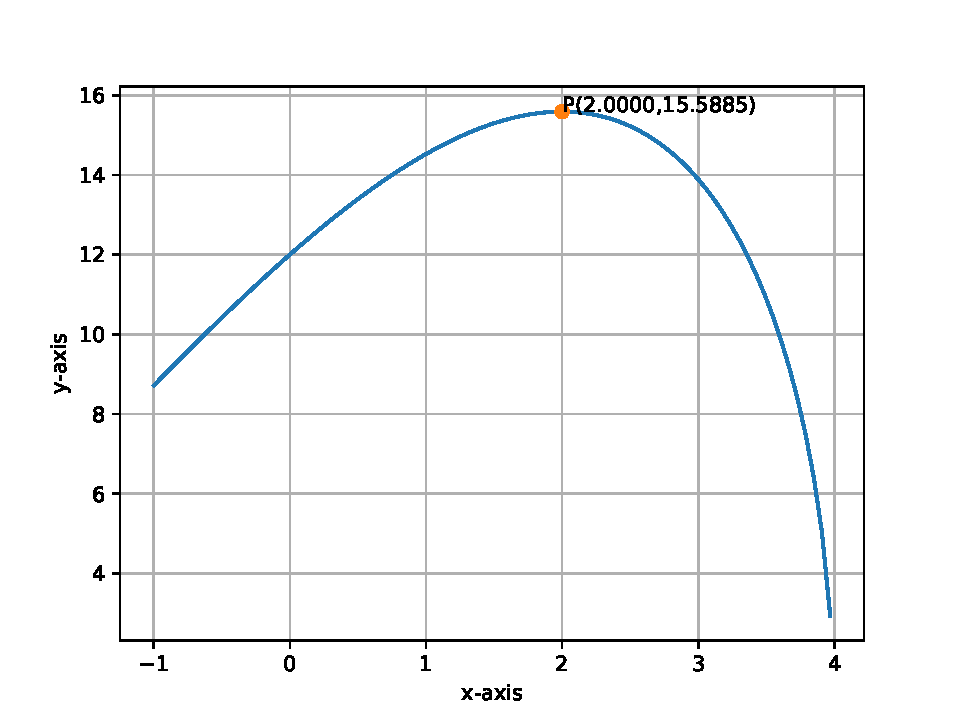
\includegraphics[width=1\columnwidth]{fig1.pdf}
	\caption{Graph of $A$ in \eqref{eq:f(x)}}
	\label{fig:graph_fx}
\end{figure}

\end{document}
